\section{Ticks, Song Stats und Hexbefehle}

Dieses Kapitel beschäftigt sich rund um das Thema Hexwerte und Hexbefehle. Es werden die meisten, aber nicht alle Hexbefehle vorgestellt, es handelt sich hierbei jedoch um die wichtigsten. \\
Unter \textit{AddmusicK/readme\_files/hex\_command\_reference.html} befindet sich eine vollständige Liste aller Hexbefehle.

\subsection*{Einschub: Hexadezimalsystem}

Das Hexadezimalsystem ist ein Zahlensystem mit Basis 16. Dabei sind die ersten 16 Ziffern (von 0 bis 15) folgende:
0, 1, 2, 3, 4, 5, 6, 7, 8, 9, A, B, C, D, E, F \\

Um eine Hexzahl von einer Dezimalzahl zu unterscheiden, kommen diese mit Präfixen daher, wie z.B. 0x oder \$. So weiß man, dass es sich bei 0x12 (gesprochen Eins Zwei) um eine 18 im Dezimalsystem und nicht eine Zwölf handelt. Mit dem Windows Taschenrechner auf Programmierer eingestellt lässt sich zudem zwischen verschiedenen Zahlensystemen bequem umrechnen.


\subsection{Ticks}

Songs die wir mit AddMusicK schreiben sind in Notenwerten, Pausen und Events zeitlich quantisiert.
Die Auflösung beträgt 48 PPQ (pulses per quarter note, deutsch Impulse pro Viertelnote) bzw. 48 TPQN (ticks per quarter note, deutsch Ticks pro Viertelnote). In FL Studio kann der PPQ Wert unter \textit{Options/Project General Settings} eingestellt werden.\\
Der kleinste zeitliche Schritt -- unabhängig vom Tempo -- ist 1 Tick. Dieser hat die Länge einer 192stel Note. Zwischen klassischen Notenwerten und Tick Werten kann also über das Verhältnis 192/Notenwert umgerechnet werden. Anstatt einem Notenwert hinter einer Note oder Pause kann mit einem Gleichheitszeichen = ein Tick Wert angegeben werden. Beispiel:

\bigskip

c2 $ \equiv $ c=96 (Rechnung: $ \dfrac{192}{c2} $)\\
r4\textasciicircum16 $ \equiv $ r=60 (Rechnung: $ \dfrac{192}{r4} +  \dfrac{192}{r16} $)\\

\bigskip

Die Auflösung von 48 PPQ hat zwei Dinge zur Folge: Unsere kleinste Note ist eine 192stel Note, eine 256stel Note ist daher nicht möglich darzustellen. Außerdem wird beispielsweise eine 128stel Note nicht richtig aufgelöst, da diese bei 48 PPQ 1.5 Ticks lang ist $(\dfrac{192}{128} = 1.5$). Stattdessen wir eine 128stel Note auf 1 Tick abgeschnitten, was wiederum einer 192stel Note entspricht. \\
Tick Werte treffen wir oft in Dateien an, die mit einem SPC/MML Konverter konvertiert wurden. Für extrem kurze Noten, beispielsweise um einen Swing Rhytmus zu erzeugen, können Tick Werte intuitiver sein als die klassischen Notenwerte.

\bigskip

Am häufigsten jedoch benutzen wir Tick Werte in Hexbefehlen. Sobald eine Dauer für einen Hexbefehl angeben wird, ist diese ein Tick Wert als Hexzahl ausgedrückt. Am Beispiel unseres Panning Befehls aus Kapitel \ref{sec:ErstenSongSchreiben} sehen wir, dass bei \$DC \$C0 \$05 die Länge \$C0 als Dezimalzahl 192 entspricht, was als Tick Wert wiederum eine ganzen Note ist. \\
Alternativ befindet sich im Anhang eine Tabelle mit einigen Längen die als Hexwerte dargestellt sind.

\subsection{Stats}

Sobald wir einen Song mit AddMusicK porten, wird automatisch im Verzeichnis \textit{AddMusicK/Stats/} ein gleichnamiges Textdokument mit verschiedenen Statistiken angelegt.

\bigskip

\begin{figure}[htbp] \centering
	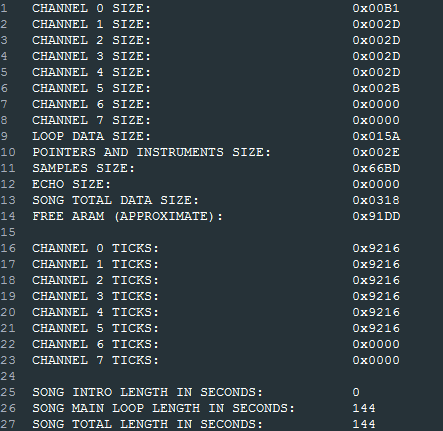
\includegraphics[width=.80\linewidth]{images/stats.png}
	\caption{Statistiken eines Songs}
	\label{stats}
\end{figure}

Channel Size 0 bis 7 geben die allgemeine Größe in Bytes als Hexwert dargestellt an,
Loop Data Size, wie viel Speicher durch das definieren der Loops selbst und deren Inhalte verbraucht wird und Pointers and Instruments Size von Pointern und Instrumentendefinitionen. \\
Die Summe dieser Werte ergibt die Total Data Size (auch Insert Size genannt) die beispielsweise angegeben werden muss, wenn ein Song auf SMW Central hochgeladen werden soll. \\
Samples Size gibt die Größe aller eingebundenen Samples und der Samples aus der Sample Group an, Echo Size von Echo, falls man diesen aktiviert.

\bigskip

Wird die Summe aus Insert Size, Samples Size und Echo Size von 64kB abgezogen (die Menge an Arbeitsspeicher vom SPC700) erhalten wir den Free ARAM (approximate) Wert, also jener Wert, der den freien Speicher im Audio Ram angibt. \\
Von diesem Wert müssen wir aber ungefähr 0x2700 Bytes abziehen (ca. 10kB), sofern keine Global Songs oder Sample Groups geändert wurden. Dieser Platz wird von der Musik Engine, Soundeffekten und Global Songs dauerhaft eingenommen und wird nicht in der Rechnung im Stats Textdokument berücksichtigt. Wird beispielsweise ein Global Song ausgetauscht, ändert sich die Grenze entsprechend.

\bigskip

Channel Ticks 0 - 7 geben die Länge der Kanäle in Ticks an, wobei es sich hierbei um Dezimalzahlen und nicht um Hexwerte handelt, trotz des fälschlicherweise verwendeten Präfixes. Im Idealfall besitzen alle verwendeten Kanäle die gleiche Länge, da der kürzeste Kanal die Gesamtdauer des Songs angibt.

\bigskip

Die letzten 3 Werte geben die Länge des Intros, des geloopten Song selbst und der Summe aus Intro und geloopten Song in Sekunden an.

\subsection{Hexbefehle}
\subsubsection{Pan Fading}
\subsubsection{Tempo Fading}
\subsubsection{Vol Fading}
\subsubsection{Pitch Bendings}
\subsubsection{Vibrato}
\subsubsection{Tremolo}
\subsubsection{Legato}
\subsubsection{Light Staccato}
\subsubsection{Echo}
\subsubsection{Yoshi Drums}